\documentclass{article}
\usepackage[utf8]{inputenc}
\usepackage{tikz,graphicx,hyperref,amsmath,amsfonts,amscd,amssymb,bm,cite,epsfig,epsf,url}

\title{big data Lecture 1: Introduction}
\author{wbg231 }
\date{January 2023}

\begin{document}

\maketitle

\begin{itemize}
    \section{big data background}
    \item here is the basic layout of a computer 
  \\  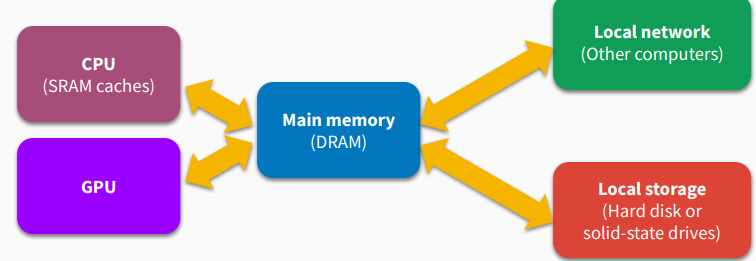
\includegraphics[width=10cm]{/home/buzgalbraith/work/school/spring_2023/big-data-spring-2023/review/week_1/lecture_1/images/l1_1.png} 
  \item we have the following resources 
  \begin{enumerate}
    \item \textcolor{red}{storage} that is where and how much data is kept
    \item \textcolor{yellow}{communication} that is how quickly can we move the data from one place to another 
    \item \textcolor{blue}{computation} how quickly can we process data 
  \end{enumerate}
  \item the cost of storage has fallen over time 
  \item both the volume of data and the speed it is created have risen over time 
  \item \href{https://www.hardwaretimes.com/difference-between-l1-l2-and-l3-cache-how-does-cpu-cache-work/}{l1 and l2 cachce} 
  \item long story short l1 is the lowest building block of the cpu it is the fastest but can not hold much data an l1 cache read takes 1 nano second 
  \item the l2 is a slightly larger piece of memory with more space, an l2 cache read takes 4 ns
  \item reading to main memory (ie dram) is the next step up and takes 100 ns 
  \item then reading from local storage (ie your hard drive) takes much larger
  \item than reading from a network takes even longer 
  \item \textcolor{red}{moore's law} the number of transistors on a micro chip (not speed) doubles every two years has widely been true 
  \item  it is wroth knowing that at this point having faster transistors is less important than having more transistors as that is where we see parallelism 
  \item we need more systems of computers not independent machines 
\section*{file systems}
\item to understand why the tools that came later developed as they did we need to go back to file systems 
\item the key ideas of file systems are using directories to organize data, and grouping structured data into files (that is data can preset across multiple runs ) 
\item  pros of file systems 
\begin{enumerate}
    \item they are easy to implement 
    \item they are portable between systems 
    \item network file systems like google drive enable limited distributed processing 
\end{enumerate}
\item file systems work well when
\begin{itemize}
    \item the data does not have obvious structure to index, then can put them in files (like for instance system logs)
    \item if indexing is not worth the cost (like one off jobs)
    \item if you are very concerned about portability between systems 
\end{itemize}
\subsection*{file system cons}
\item they do not expose or exploit structure of the data
\item each query requires a new program is written (hard to re use)
\item directories and hierarchies may be too restrictive (like if we have files that are conceded in some non obvious way )
\item file systems are bad when 
\begin{itemize}
    \item the data is structured along multiple axes 
    \item when the data has complex interactions 
    \item when analysis is complex
    \item when the benefits of indexing data outweigh the costs. 
    \item in cases like this we can use the relational database model
\subsection*{methods for dealing with large datasets in a file system}
\item sample ie just take part of the files or a piece of a file 
\item stream processing look one record at a time 
\item data structures (is using an RDD a good idea)
\item indexing (sorting data so looking up records is fast)
\item parallelism 
\end{itemize}
\item it is wroth noting that databases did not replace file systems 
\item file archives are still a common way to share large datasets (but we include metadata to show how that data is structured)
\item hadoop relies on a distributed file system, then you build database abstractions on top, but this comes with restrictions on structure 
\item so the key difference today is that \textcolor{blue}{ we use standardized file formats}
\subsection*{things to consider when choosing what tool is best }
\item do you need an exact solution to the problem (is an approximation good enough ) if so may only need part of the data
\item di we expect records to be wrong?
\item will the dataset grow over time?
\item will the number of features we are looking at ever change?
\item how complex is the way we are doing things?
\subsection*{slido}
\item Say you had to compute the mean and
covariance matrix of a "large" collection of
100-dimensional vectors. How would you
rank the above strategies (best to
worst)?
\item sampling will give you an approximation but may miss outliers
\item stream processing will limit memory usage but not CPU time 
\item indexing does not help: this problem uses all the data 
\item parallelism will work if you have access to many machines 
\item a good approach would b eto stream first to limit memory usage (which is always helpful) then either use parallelism or sampling depending on if an approximation is ok 
\subsection*{what is next}
\item data base management systems (DBMS) they provide a standardized interface to store load and process data. 
\item that relation mode which imposes constraints on how the data is organized but gives us speed ups 
\item putting these two ideas together yields the relational data base model (RDBMS)
\end{itemize}

\end{document}
